\documentclass[12pt]{jreport}
\usepackage[dvipdfmx]{graphicx}
\input{jdummy.def}
%卒論用スタイルファイル
\usepackage{jgraduate2015_sjis}
%索引作成用
\usepackage{makeidx}
\usepackage{graphicx}
\usepackage{ascmac}
\usepackage{enumerate}
\usepackage{comment}
\usepackage{url}
\usepackage{cite}

% 前設定
\date{平成27年2月}
\title{WLANとZigBeeの共存に向けた\\AP-Assisted CTS-Blockingに関する研究}
\author{佐伯 良光}
\university{九州大学大学院}
\department{システム情報科学府}
\course{修士課程}
\major{情報知能工学専攻}
\subcourse{社会情報システム工学コース}

\begin{document}

%表紙
\maketitle

\begin{abstract}
% 概要
現代社会において,無線ネットワークによる通信は生活に不可欠な存在である.
特に近年,無線LAN(Wireless LAN,WLAN)通信はモバイル端末の普及などの要因も
あり,広く一般に利用されている.
一方,別のネットワーク通信としてZigBeeが注目されている.
ZigBee端末は他の無線ネットワーク端末に比べ安価で省電力であるため,
センサネットワークを用いたM2M(Machine to Machine)技術に利用される.

しかしながら,WLANとZigBeeでは同一の周波数帯を利用するため,
干渉が発生し通信が阻害されるため共存が難しい.
そこで,同一周波数帯を利用するWLANとZigBeeの共存に向けて
容易に構築可能な衝突回避方式の研究を行っている.
衝突回避方式の実現に向けては既存の機器をそのまま利用できることが必要となることから,
OSやハードウェアの改変を必要としないシンプルな方式の実現が重要となる.

本論文ではこのような観点で設計された
AP-Assisted CTS-Blocking(AA CTS-Blocking)方式を示す.
AA CTS-Blocking方式ではRTS/CTS方式を応用することでWLANの通信を抑制し,ZigBee通信と
WLAN通信の衝突を回避させる.
RTS/CTS方式はWLANの標準に定められた衝突回避機構であり,所定の手順を踏んで
RTS/CTSフレームを送信することでOSやハードウェアの改変を行うことなく
WLANとZigBeeの衝突を抑制することができる.
AA CTS-Blocking方式を適用したZigBeeデータ収集システムを実装し,
実証評価を通じてAA CTS-Blocking方式の衝突回避効果により
ZigBee通信の成功率が向上したことを確認した.


\end{abstract}


%目次
\tableofcontents

\newpage

%ページ番号をアラビア数字に
\pagenumbering{arabic}


\chapter{はじめに}\label{intro}%==============================================
%WLAN利用例を示し,WLANが普及していることを示す.分量もう少し増やす(後ほど)
現代社会において,無線ネットワークによる通信は生活に不可欠な存在である.
特に近年,無線LAN(Wireless LAN,WLAN)通信はWi-FI等で広く一般に普及している.
例えばPCとプリンタを,自宅のWLANアクセスポイント(Access Point,AP)に接続し
印刷を行うことは珍しくない.
それだけにとどまらず,更にHDD,テレビ,レコーダーなど,様々なデジタル機器を
WLANネットワークに接続して利用するホームネットワークという概念も登場している.
近年では,WLAN通信端末の主体がスマートフォンやタブレットで代表される
モバイルワイヤレス端末に移行しつつある.
コンビニエンスストアや駅など,不特定多数の人々がゲストとしてアクセス可能な
WLAN APの設置も進んでいる.
特定の場所に限らず,あらゆる地域・場所でWLANネットワークに
接続して通信することが求められるようになってきている.

%ZigBee利用例を示し,ZigBeeがこれから増えていくことを示す.分量もう少し増やす(後ほど)
他方で,別のネットワーク通信としてZigBeeが注目されている.
ZigBeeとは,IEEE 802.15.4に準拠したセンサーネットワークを主目的とする
近距離無線通信規格の1つであり,WLANに比べ通信距離が短く通信速度も
低速であるが,安価で省電力である.
それ故に,ネットワークに繋がれた機器同士が人間を介在せずに通信し,
サービスを提供するM2M(Machine to Machine)技術によく利用される.
M2Mの応用範囲は非常に幅広く,多様なサービスを提供可能である.
屋内にZigBeeネットワーク接続されたセンサを配置して,
電力やガスの消費量や,温度を最適に自動制御するスマートハウスもM2Mの1つである.

%干渉の話分量もう少し増やす(後ほど)
ネットワーク技術の進歩に伴い人々の暮らしが益々便利になる
一方で,通信フレームの衝突による干渉という課題も存在する.
例えば,ZigBeeセンサにより構築されたスマートハウスを利用する場合,
屋内にWLAN APが存在すれば干渉が発生する可能性は高い.
干渉とは,電波技術Aに対応した受信機Txが電波Aと電波Bの混在した電波を受信した際,
正常に電波をデコードできないことを指す.
これはZigBeeが,WLANと同じ2.4GHz帯を利用するためである.
図\ref{fig:frequency}に,WLAN及びZigBeeの周波数チャネルを示す.
ZigBeeのすべてのチャネルはWLANの複数のチャネルと重なっており,
ZigBeeとWLANの中心周波数が近いところでは相互に干渉が生じる
ことが報告されている~\cite{shuaib06:wifi_zigbee}.
WLANはZigBeeに比べて10〜100倍程度送信電力が大きいため,
干渉による通信への影響はZigBee側が大きい.

\begin{figure}[bt]
 \centering
 \includegraphics[width=\columnwidth]{figure/frequency.pdf}
 \caption{WLAN及びZigBeeの周波数チャネル}
 \label{fig:frequency}
\end{figure}

WLAN,ZigBeeにはアクセス制御方式としてCSMA/CA
(Carrier Sense Multiple Access / Collision Avoidance)機構を具備している.
しかし,WLANのCSMA/CAではWLANのみの通信環境,
ZigBeeのCSMA/CAではZigBeeのみの通信環境を想定しているため,
WLAN通信とZigBee通信が混在した環境において互いの干渉を回避することは困難である.

WLAN通信とZigBee通信が混在した環境内におけるWLANとZigBeeの共存を目的とした干渉回避方式として,
文献~\cite{hou09:minimize_intf}ではWLANのアクセス制御であるRTS/CTS(Request to Send / Clear to Send)方式
を利用したCTS-Blockingが提案されている.
図\ref{fig:cts_blocking}に,CTS-Blockingの概要を示す.
CTS-Blockingでは,制御PCからCTSフレームを直接送信することで周囲の
WLAN端末の通信を一時的にブロックする.
WLAN通信において,送信端末以外の端末がCTSフレームを受信すると
CTSフレーム内の\texttt{Duration}フィールドに記載された時間だけ送信を控える.
CTS-Blockingではこれを利用して周囲のWLAN端末の
通信を抑制し,WLANとZigBeeの干渉を回避する.
しかしながら,現在のOS・無線LANモジュールでは通信の公平性確保の観点からCTS
フレームの直接送信が禁止されており,CTS-Blockingの実現に向けてハードウェアや
OSの改変が必須となる.
また,送信電力制御の影響によりCTSフレームの到達範囲が狭くなる可能性があり,隠れ端末問題の影響を受けやすい.

WLANとZigBeeの共存のためには,
ハードウェアやOSを改変することなく,
既存のモジュールをそのまま用いてWLANからの干渉を受けないZigBee通信を実現する
ことが重要である.
これに向け,筆者らは既存のRTS/CTS方式をそのまま利用した
AP-Assisted CTS-Blocking(AA CTS-Blocking)干渉回避方式の開発を進めている.
本稿では,AA CTS-Blocking方式について述べ,その有効性の検証に向けた実証評価について報告する.

\begin{figure}[bt]
 \centering
 \includegraphics[width=\columnwidth]{figure/cts_blocking.pdf}
 \caption{CTS-Blockingと隠れ端末問題}
 \label{fig:cts_blocking}
\end{figure}

本論文の構成は以下の通りである.
\ref{fundamental}章ではWLAN及びZigBeeの基礎技術について触れ,アクセス制御方式などの説明を行う.
\ref{relation}章ではWLANとZigBeeの共存に向けた干渉回避方式に
関する研究について述べ,既存システムの課題を示す.
\ref{aa_cts}章では筆者らが提案するAA CTS-Blocking方式の概要及び設計について示す.
\ref{imple}章ではAA CTS-Blocking方式を適用した
ZigBeeノードによるデータ収集システムの実装について述べ,
\ref{eval}章でWLAN通信環境下におけるZigBeeノードによるデータ収集システムについて,
AA CTS-Blocking方式の有無による通信成功率の差を比較・考察する.
最後に\ref{conclu}章でまとめとする.

\chapter{WLAN及びZigBeeにおけるネットワーク・プロトコル}
\label{fundamental}
%====================================================================
本章における研究対象を明確に示すため,ネットワーク上での通信に関する規約を
定めたものであるネットワーク・プロトコルについて説明を行う.
2.1節では現在の標準であるTCP/IPプロトコルについて簡単に触れる.
2.2節ではTCP/IPのうちリンク層におけるMACについて示し,
2.3節ではWLANのMACを策定しているIEEE 802.11及び,
ZigBeeのMACを策定しているIEEE 802.15.4(-2003)を説明する.
2.4節では本研究に深く関連する,IEEE 802.11及びIEEE 802.15.4で規定されている
具体的なアクセス制御方式について紹介する.\\

%この研究がどの階層(レイヤ)のものなのかを述べる.key:2.1 TCP/IP参照モデル,2.2 IEEE 802.11,2.3 IEEE 802.15.4など
\section{TCP/IP}

TCP/IPとは,インターネットなどで標準的に用いられる通信プロトコルであり,TCP\\
%TCP(Transmission Control Protocol)とIP(Internet Protocol)を組み合わせたものである.
(Transmission Control Protocol)とIP(Internet Protocol)を含むインターネット標準のプロトコル群全体の総称である.
IPは複数のネットワークを繋ぎあわせて相互に通信可能にするプロトコルである.
現代社会において欠かすことのできないインターネットも,
IPを用いて世界中の様々な組織の管理するネットワークを相互接続してできたものである.
%オープンなネットワークのことである.
TCPはIPを基盤にその上層で利用されるプロトコルで
IPネットワーク上の2地点間で信頼性の高い通信を可能にする.

\begin{comment}
TCPのさらに上層では,用途やソフトウェアに応じて様々なプロトコルが規定されている.
例えば,WebではHTTP(HyperText Transfer Protocol)が用いられるが,
HTTPはTCPを、TCPはIPをそれぞれ利用してデータを転送している.
インターネットなどのIPネットワークではIPと組み合わせてTCPではなくUDPなどが用いられることもあるが、「TCP/IP」という呼称はTCPとそれ以外を区別するという意味合いは薄く(「UDP/IP」という言い方はほとんどしない)、「IPを中心とする標準的な通信プロトコルの総称」を表すことが多い。歴史的な経緯からそのような用法が定着しているが、今日ではそのような総称的な意味は「インターネットプロトコルスイート」(Internet Protocol Suite)のような用語で表すべきとされることもある。
\end{comment}

\section{TCP/IP参照モデル}

TCP/IPプロトコル群は階層の一式として見ることができる.
図\ref{fig:tcp_ip_ref_model}にTCP/IP参照モデル,OSI参照モデル及び
それに関連したプロトコルなどを示す.
TCP/IP参照モデルは4つの階層で構成される.

\begin{figure}[bt]
 \centering
 \includegraphics[width=\columnwidth]{figure/tcp_ip_ref_model.pdf}
 \caption{TCP/IP参照モデル及びOSI参照モデル}
 \label{fig:tcp_ip_ref_model}
\end{figure}

実際にTCP/IPプロトコル群を利用して通信を行う時,各階層ではデータにヘッダを付加する.
データは付加されたヘッダの情報をもとに,送信先や送信先で引き渡すアプリケーションなどの判断を行う.
ヘッダとは〜である.
具体的な通信の流れとして,図\ref{fig:tcp_ip_comm}にTCP/IP参照モデルを用いた通信例の説明を示す.
データの流れとしては各層へ逐次的に通信を行い,ヘッダを付加する.
送信元ではアプリケーション層からトランスポート層,インターネット層を通ってネットワークインターフェース層まで通信を行う.
ネットワークインターフェース層ではハードウェアである通信ケーブルへデータパケットを送信し,
受信先では送信元とは逆順でネットワークインターフェース層からインターネット層,トランスポート層を通りアプケーション層へと至る.
以下でTCP/IP参照モデルにおける各層の役割について詳細を示す.

\begin{figure}[bt]
 \centering
 \includegraphics[width=\columnwidth]{figure/tcp_ip_comm.pdf}
 \caption{TCP/IP参照モデルによる通信の説明}
 \label{fig:tcp_ip_comm}
\end{figure}

データリンク層はネットワークコミュニケーション層とも呼ばれ,データリンクプロトコルを利用して
通信をするためのインターフェースとなる階層である.
具体的なイメージとしては,PCやスマートフォン等のハードウェアとOS間で
データの橋渡しをするような役割を持つ.
データリンクプロトコルの例として,イーサネット,IEEE 802.11,WLAN等があり,
本研究とも関連が深い.

ネットワーク層は,IPプロトコルを使用して付加する
IPアドレスをもとにしてデータパケットの転送を行う階層である.
IPにはデータリンクの特性を隠す役割もあり,通信したいホスト間の経路が
どのようなデータリンクプロトコルを用いていたとしても通信が可能である.
故にインターネットを利用して通信を行うことが可能であり,
インターネットに接続する機器では必ずIPの機能が実装されている.

トランスポート層はアプリケーションプログラム間の通信を実現する階層である.
PCの内部では複数のプログラムが同時に動作しているため,
どのプログラムとどのプログラムが通信しているかを識別する必要がある.
トランスポート層におけるプロトコルでは,
アプリケーションプログラムを識別するために,ポート番号と呼ばれる識別子が使われる.
TCP/IP参照モデルにおいては,
前述したネットワーク層及びトランスポート層はOSに組み込まれることが想定されている.

アプリケーション層はトランスポート層より上の階層であり,アプリケーションプロセスのための
共通アプリケーションサービスへ直接接続して実行したり,
OSI参照モデルの第6層であるプレゼンテーション層に対して要求も行うなど,役割の幅が広い.
共通アプリケーション層サービスとは関連するアプリケーションプロセス間の意味的な変換を提供するものであり,
一例としては,仮想ファイル,仮想端末,ジョブの転送及び操作プロトコルなどである.
アプリケーション層に属するプロトコルの例としては,
ブラウザ - サーバー間の通信で使われるHTTP(HyperText Transfer Protocol)や
暗号や認証の技術を利用して,安全にリモートコンピュータと通信するためのSSH(Secure Shell)などがある.

各層はデータ転送に伴い生じる一連の問題を解決し,
下位層プロトコルのサービスを使用する上位層プロトコルに明確なサービスを提供する.
上位層は利用者と論理的に近く,より理論的なデータを処理する.
また最終的に物理的に転送できる形式へデータを変換するため,下位層プロトコルに依存する.
本研究で取り扱うのは最下層であるデータリンク層である.
次節で,WLAN及びZigBeeの準拠するIEEE 802における通信プロトコルである,
データリンク層に属するMAC(Media Access Control)について説明する.

\section{Media Access Control}
\label{sec:mac_protocol}

Media Access Controlは日本語で媒体アクセス制御またはメディアアクセス制御といい,
IEEE 802におけるTCP/IPモデルの第1層にあたるデータリンク層の一部を成す通信プロトコルである.
MAC は,データリンクに接続しているノードを識別するために利用するアドレスを指定する.
これをMACアドレスといい,各ネットワークカードに割り当てられた固有の番号であり,
サブネットワーク(イーサネットなどのルーターを経由しない物理ネットワーク)内の通信相手にパケットを送信可能とする.
この様に,MAC層は論理リンク制御とネットワークの物理層の間のインタフェースとして動作し,
物理アドレスあるいはMACアドレスによるアドレッシング機構を提供する.

また,MACは複数の無線ネットワーク端末が電波帯域を共有して情報を送る
多元接続を制御する機構を提供する.
従って複数のターミナルやネットワークノードをネットワーク上で通信可能とし,
一般にLocal Area Network(LAN)やMetropolitan Area Network(MAN)で使用される.
\ref{sec:multiple_access}項でこの多元接続の制御方式について説明し,
\ref{sec:multiple_access}項でWLANにおけるMACプロトコルを,

%全二重の一対一の通信では、MACプロトコルは必要とされない。
%半二重の一対一の通信では、全二重のエミュレートが可能であり、その際にMAC層を使うこともある。
%MAC層は論理リンク制御とネットワークの物理層の間のインタフェースとして動作し,
%物理アドレスあるいはMACアドレスと呼ばれるアドレッシング機構を提供する.
%これは各ネットワークカードに割り当てられた固有の番号であり,
%サブネットワーク(イーサネットなどのルーターを経由しない物理ネットワーク)内の通信相手にパケットを送信可能とする.
%媒体アクセス制御という用語は多元接続プロトコルと同義に使われることもある。
%というのも、MAC層は多元接続に必要なプロトコルと制御機構を提供するためである。
%これにより、複数の局が同じ物理媒体を共有することが可能となる。
%物理媒体共有の例として、バス型ネットワーク、リング型ネットワーク、ハブ型ネットワーク、無線ネットワーク、全二重の一対一リンクなどがある。

\subsection{多元接続制御方式}
\label{sec:multiple_access}

無線ネットワークでは,周波数帯域は限られたリソースであるため多元接続に対する制御方式が必要になる.
多元接続制御方式として代表的なのは,図\ref{fig:multiple_access}に示す
周波数分割多重方式(Frequency Division Multiple Access,FDMA),
時分割多重方式(Time Division Multiple Access,TDMA),
時分割多重方式(Code Division Multiple Access,CDMA),
の3つである.
以下にその詳細を示す.

\begin{figure}[bt]
 \centering
 \includegraphics[width=0.8\columnwidth]{figure/multiple_access.pdf}
 \caption{多元接続制御方式}
 \label{fig:multiple_access}
\end{figure}

FDMAは,電波の周波数帯を複数の帯域に分割することで多元接続を行う無線通信技術である.
各無線局にはそれぞれ異なる搬送周波数が割り当てられる.
要求割当多元接続 (DAMA : Demand Assigned Multiple Access) の場合,接続確立時と終了時になんらかの制御機構を必要とする.
その結果,任意の部分帯域をどの地球局にでも割り当て可能となる.
FDMA には要求割当の他に固定割当 (PAMA : Pre-Assigned Multiple Access) もある.
要求割当は,統計的割当処理を使って一時的に搬送周波数を割り当てることで
全てのユーザーに対してトランスポンダの帯域への連続なアクセスを可能とする.

TDMAは,同一周波数の電波の固定タイムスロットをそれぞれの無線局に割り当て多元接続を行う無線通信技術である.
特徴としては,時間ダイバシティが使用できるためフェージング耐性があり,回線交換接続が可能で遅延時間や通信速度が保証できる.
但し,無線局間の同期が必要不可欠である.
TDMAにおける周波数利用効率・回路規模は,FDMAとCDMAの中間程度である.
時間軸圧縮を行っているため音声の場合遅延時間があるが,通信衛星を利用する場合には
FDMAと比較して地球局から受信する電波の電力の差に対応しやすい.

CDMAは,複数の発信者の信号にそれぞれ異なる符号を乗算し,すべての信号を合成して
1つの周波数を使って送信し多元接続を行う無線通信技術である.
主に直接拡散符号分割多重接続 (DS/CDMA,DS : Direct Sequence),周波数ホッピング (FH : Frequency-Hopping) の方式に分けられる.

CDMAでは,Cell BreathingというCDMA基地局の通信範囲(セル)の大きさが呼吸しているように収縮変化する特有の現象が存在する.
Cell Breathingは,FDMA,TDMAでは見られない.
CDMAの場合,セル内の端末は同一周波数で通信するため常に干渉(お互い混信している)状態にあるが,
セル内の端末数が増えて容量の限界に近づいてくるとエリア端に近い局は電波伝播損失が大きいため,
基地局に近い局よりも干渉量が大きくなり基地局との通信が出来なくなる.
この現象をマクロで見ると,あたかもセルの大きさが収縮しているように見えるためCell Breathingという.
%また,端末の台数により

\subsection{WLANにおけるMACプロトコル}
\label{sec:ieee_ 802.11}

WLANの規格であるIEEE 802.11bやIEEE 802.11gではアクセス制御方式としての通信プロトコルが
いくつかあるため,本稿ではそれらについて説明する.
IEEE 802.11は,米国電気通信学会IEEE(The Institute of Electrical and Electronics Engineers, Inc.)により策定された
広く普及しているWLAN関連規格の1つであり,1997年に初めて規格統一されたWLAN規格であるIEEE 802.11をはじめとして
現在では\ref{fig:wlan_assort}に示す8つの規格が存在する.
このうち,IEEE 802.11a,IEEE 802.11b及びIEEE 802.11gにおいて利用されているのが
CSMA/CA(Carrier Sense Multiple Access/Collision Avoidance,搬送波感知多重アクセス/衝突回避方式)である.
そのシーケンスを図\ref{fig:csma_ca_wlan}に示す.
CSMA/CAでは,まず通信を開始する前に一度受信を試みることで現在通信をしているホストが他にあるかどうか確認する,
搬送波感知(Carrier Sense)を行う.
WLAN環境中は複数のWLAN端末が同じ回線を共用しているため,多重アクセス(Multiple Access)状態である.
搬送波感知の結果,他者が通信をしていなければ自分の通信を開始する.
ここで搬送波感知の段階で通信中のWLAN端末が存在した場合,通信終了と同時に送信を試みると衝突する可能性が高い.
従って,他のWLAN端末の送信終了を検知した場合は自分が送信を開始する前にランダムな長さの待ち時間をとる.
なお、永久に送信できない事態を防ぐため、この待ち時間は徐々に短くされてゆく。
これが衝突回避(Collision Avoidance)部分にあたる.

\begin{figure}[bt]
 \centering
 \includegraphics[width=\columnwidth]{figure/csma_ca_wlan.pdf}
 \caption{WLAN環境におけるCSMA/CA方式}
 \label{fig:csma_ca_wlan}
\end{figure}

しかし,CSMA/CAでは図\ref{fig:hidden_device}に示す隠れ端末問題を解決できない.
隠れ端末問題とは,無線通信において互いに相手の通信を検知できない関係にある複数の機器が
同じ機器に向けて同時に信号を送信してしまい,信号の衝突(コリジョン)が発生してしまう問題である.

\begin{figure}[bt]
 \centering
 \includegraphics[width=\columnwidth]{figure/hidden_device.pdf}
 \caption{隠れ端末問題}
 \label{fig:hidden_device}
\end{figure}

IEEE 802.11においては,
RTS(Request to Send)/CTS(Clear to Send)方式を採用しており,これを用いて隠れ端末問題による
干渉の影響を軽減している.
RTS/CTS方式のシーケンスを図\ref{fig:rts_cts}に示す.
WLAN環境におけるRTS/CTS方式では送信電力の大きく通信範囲の広いAPを利用するため
周囲の多くのWLAN端末にCTSフレームが届き,
CSMA/CA方式より確実なアクセス制御を行うことが可能であるが,
送信前に必ず待ち時間が入るため,オーバーヘッドが生じる.

\begin{figure}[bt]
 \centering
 \includegraphics[width=0.8\columnwidth]{figure/rts_cts.pdf}
 \caption{WLAN環境におけるRTS/CTS方式}
 \label{fig:rts_cts}
\end{figure}

\subsection{ZigBeeおけるMACプロトコル}
\label{sec:ieee_ 802.15.4}

ZigBeeの規格であるIEEE 802.15.4ではIEEE 802.11同様,アクセス制御方式としての通信プロトコルは
CSMA/CAを利用している.
図\ref{fig:csma_ca_zigbee}にその動作の詳細を示す.
%但し,詳細な動作は少し異なるため,以下でそれを示す.
%図\ref{fig:csma_ca_zigbee}に示す,IEEE 802.15.4におけるCSMA/CAでは,
%〜

\begin{figure}[bt]
 \centering
 \includegraphics[width=\columnwidth]{figure/csma_ca_zigbee.pdf}
 \caption{ZigBee環境におけるCSMA/CA方式}
 \label{fig:csma_ca_zigbee}
\end{figure}


\chapter{関連研究及びその比較}\label{relation}%==============================================

干渉回避方式に関する研究は膨大に存在するが,
大別すると
\begin{enumerate}

 \item WLAN/ZigBeeの既存のアクセス制御方式を利用した\\
 方式~\cite{hou09:minimize_intf,zhang11:zigbee_wifi_coexist,murata14:wlan_zigbee,huang09:wlan_zigbee,tytgat12:wlan_zigbee}

 \item 既存のアクセス制御方式以外の技術を利用した
 方式~\cite{huang10:beyond_coexist,liang10:wifi_zigbee_survive}

\end{enumerate}
に分類される.

WLANのCSMA/CA機構を利用した干渉回避方式としてCBT~\cite{zhang11:zigbee_wifi_coexist}が挙げられる.
CBTでは,
signalerと呼ばれるZigBeeノードをWLAN機器の近くに配置し,ZigBee通信時にsignalerから
長いフレームを送信することでWLAN端末にZigBeeが通信状態にあることを通知する.
WLAN端末ではsignalerの送信信号によりCSMA/CA機構が働き,送信が抑制されるため
WLANとZigBeeの衝突を回避できる.
しかしながら,
スマートフォンなどの移動体も含めて考えると
全てのWLAN機器の近くにsignalerを配置することは非現実的である.

また,村田ら~\cite{murata14:wlan_zigbee}は干渉の原因をZigBeeのaTurnaroundTime(送受反転時間)が
通信アイドル時の待機時間であるDIFS(DCF Inter Frame Space)よりも長いことと捉え,
DIFSを拡大する方式を提案している.
DIFSをaTurnaroundTimeに比べ長くとることで衝突を回避する.
しかしながら,DIFSを拡大するためには予めAPにアクセスして設定しなければならず,
実現のためには周囲のAP全てを管理下に置かなければならない.

ZigBeeが準拠しているIEEE 802.15.4のビーコンモードによるアクセス制御を利用した
干渉回避方式も提案されている~\cite{huang09:wlan_zigbee}.
Dynamic GTSでは,ビーコンモードの1つである
ZigBeeノードにGuaranteed Time Slot(GTS)を割当て優先的に通信できる期間CFP(Contention Free Period)
を利用し,このCFPを拡大することで衝突を回避する.
CFPの拡大は,GTSを動的に配置しそのビーコンを検知したWLAN端末が
CTSフレームを送信することで達成可能である.
しかしながら,\ref{sec:intro}で示したCTS-Blockingと同様に
ハードウェアやOSの改変が必須である点,
隠れ端末問題の影響を受けやすい点が問題である.
CACCA~\cite{tytgat12:wlan_zigbee}においても同様の問題が考えられる.

既存のアクセス制御方式以外の技術を利用した方式として,
無線通信の通信空き時間を有効活用して通信を行うための「White Space」技術
を応用した干渉回避方式が提案されている~\cite{huang10:beyond_coexist}.
WISEでは,WLAN通信におけるWhite Spaceを予測し,そのWhite
Space内で通信が完了するようにZigBeeフレーム長の動的制御を行う.
例えば,WLAN通信の混雑時には予測されるWhite Spaceの長さは短くなるため,
ZigBeeノードにおいてデータを分割して送信する.
これにより,ZigBeeフレームがWLAN通信によって破壊される確率を低減させるこ
とが可能となる.
しかしながら,WLAN通信が混雑している時にはWLAN通信の空き時間が少ないため
にWhite Spaceの予測が外れ,通信が衝突する確率が高くなる.

フレーム衝突について分析し,分析結果を干渉回避方式とした研究もある.
BuzzBuzz~\cite{liang10:wifi_zigbee_survive}では,WLANとZigBeeのフレーム衝突により通信が阻害される原因として
IEEE 802.15.4フレームのヘッダが破壊されることと捉え,
ヘッダを2重にして送信することでZigBeeのパケットロス率を減少させている.
BuzzBuzzはこれまでに紹介した関連研究群とは違い,
既存の方式やモジュールの改造及び特別なハードウェア等の利用が必要なく,
干渉回避方式の構築コストについて考慮されている.
これは,本稿で提案するAA CTS-Blocking方式とは違うアプローチで
ZigBeeの通信を保証しており,
AA CTS-Blockingと組み合わせることでさらなる干渉回避効果が期待される.

%--------------------------------------------------

%----------------------------------------------------------------------
\chapter{AP-Assisted CTS-Blocking方式の提案}
\label{aa_cts}

WLAN APは,WLAN端末に比べ送信電力が
大きく,RTS/CTS制御方式においても利用されるため,
これを利用して干渉回避方式であるAP-Assisted(AA)
CTS-Blockingを提案する.

\section{概要}
\label{sec:outline}

図\ref{fig:aa_cts_blocking}に,AA CTS-Blocking方式の概要を示す.
本システムは,環境内に配置された複数のZigBee End Device(ZED)及び
ZigBeeネットワーク制御を行うZigBee Coordinator(ZC),制御PCから構成される.
ZigBee基地局と制御PCは有線接続されている.
AA-CTS Blockingでは,周辺にあるWLAN APからCTSフレームを送信させることでWLAN通信をブロックし
干渉の影響を低減したZigBeeノード間の通信を実現する.

\begin{figure}[bt]
 \centering
 \includegraphics[width=\columnwidth]{figure/aa_cts_blocking.pdf}
 \caption{AA CTS-Blocking}
 \label{fig:aa_cts_blocking}
\end{figure}

\figurename~\ref{fig:sequence}にAA CTS-blocking方式の
通信シーケンスを示す.
制御PCは,あらかじめ周囲に存在するWLAN APのビーコンフレームを受信し,
チャネル,受信信号強度(RSSI)等を収集しておく.
ZigBeeノード間の通信を行う場合,まず(1)~制御PCはAPを1つ選択し,
(2)~制御PCは選択したAPに向けてRTSフレームを送信する.
次に(3)~RTSフレームを受信したAPは
周囲のWLAN端末に向けCTSフレームをブロードキャストする.
CTSフレームを受信したWLAN端末はCTSフレーム内の\texttt{Duration}
フィールドに記載された時間だけ送信を控えるため,WLAN通信が一時的にブロックされる.
WLAN通信Block期間(Duration of Block WLAN Communication,DBW)がスタートした時,
(4)~CTSフレームを受信した制御PCは,有線接続されたZCに向けて通信開始信号
(Communication Start Signal,CSS)を送信することで
ZigBeeノード間の通信を開始する準備が整う.
ZigBeeノード間の通信は
ZCを用いた制御によりDBW内に完了させる.

このようなAA CTS-Blockingを実現する上では2つの疑問が生じる.
\begin{enumerate}
 \item RTS送信先APをどのように選ぶか
 
	実環境には多くのWLAN APが存在するため,
	制御PCはRTSの送信先APを選択する必要がある.
	\ref{ssec:select_ap}において,周囲に存在するWLAN APのビーコンフレームを用いた
	AP選択アルゴリズムを示す.

 \item DBWにおいて,ZigBeeノード間通信をどのようにスケジューリングするか
 
 	DBWは有限であるため,
	ZigBeeノード間で通信の衝突が起きないようアクセス制御を行う必要がある.
	\ref{ssec:design}において,1台のZCと複数のZEDとの通信における
	スケジューリング手法を検討する.

\end{enumerate}

\begin{figure}[bt]
 \centering
 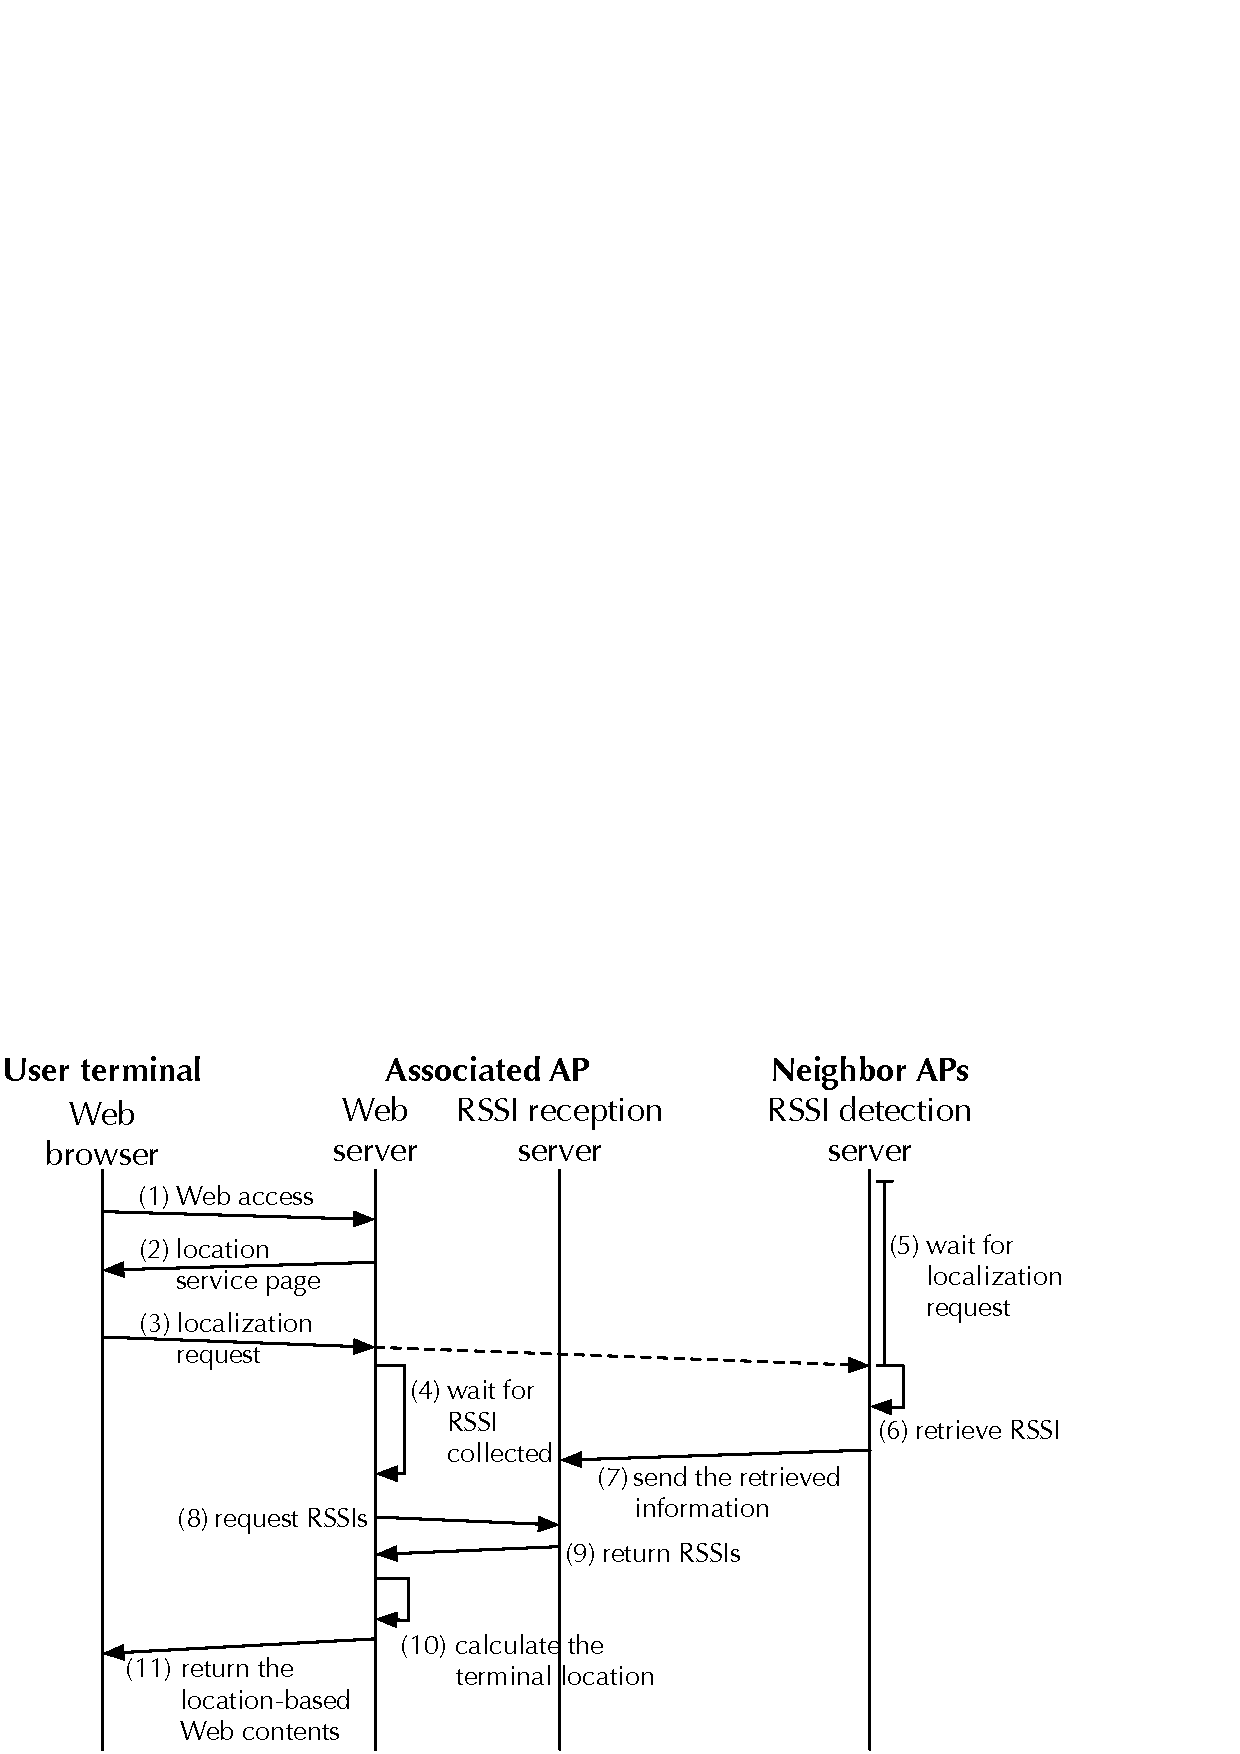
\includegraphics[width=\columnwidth]{figure/sequence.pdf}
 \caption{AA CTS-blocking方式の通信シーケンス}
 \label{fig:sequence}
\end{figure}

\section{AP選択アルゴリズム}
\label{ssec:select_ap}

AA CTS-Blockingにおいては,RTSフレームの送信先APの選択は
干渉回避性能に大きな影響を及ぼす.
例えば,制御PCの通信可能範囲ギリギリの位置に存在するAPを選択した場合
RTSフレームがAPに届かない可能性やAPからのCTSフレームを受信できない可能性がある.
RTSフレーム送信先APの選択を最適化することにより,
より確実により多くのWLAN通信をブロックできる.

本研究ではAPと制御PCの物理的距離が重要になると考え,
位置推定~\cite{izumi13:awpn_acc_imprv}などにも用いられる
RSSIをAP選択アルゴリズムのキーとして採用した.
RSSIの取得は特殊なパラメータや追加のデバイスを必要とせず,
既存のAPから発せられるWLANフレームを受信するだけで収集可能である.
図\ref{fig:aa_cts_blocking}に示すように制御PCがZCに有線接続されており,
ZEDはZCを中心に周囲に配置されていることも考慮に入れると,
制御PC周辺のWLAN通信をブロックすることが非常に有効であると考えられる.

\section{スケジューリング手法}
\label{sec:design}

AA CTS-Blocking方式においては,ZigBeeノード間の通信はAPから送信されたCTSフレーム内の
\texttt{Duration}フィールド(最大値は32\,ms~\cite{IEEE802_11-2007})に記載された時間内に終了させる
必要がある.
ZEDの台数が増えた場合通信回数が増え,1回のRTS/CTS送信での通信が難しくなるため,
スケジューリング等のアクセス制御方式が必須となる.

これに向け,本研究では既存のMACプロトコルを利用する.
MACプロトコルは種類を問わず利用可能である.
ZEDの台数が32\,ms間で通信できない台数に増加した場合には,
ZEDをグループ化し,ZCからの制御によってRTS/CTSの1回の送信に
対して1グループに通信を許可すれば良い.
ただし,グループ間での通信に関しては問題が残る.
これについては今後の研究課題とする.

一例として,TDMA(Time Division Multiple Access)方式のMACプロトコルを利用する場合,
\ref{ssec:outline}で示したZigBeeノード間の通信シーケンス部分は以下のようにすれば良い.
制御PCからCSSを受信したZCは,周囲のZEDへデータ要求フレームをブロードキャストする.
データ要求フレームを受け取ったZEDは,
データ要求フレームをSlot同期信号としてTime Slot(TS)を用いたアクセス制御を開始し,
ZED毎にあらかじめ定められたSlotにおいてZCに対してデータフレームを送信する.

%----------------------------------------------------------------------
\chapter{設計及び実装}
\label{imple}

本章では,AA CTS-Blocking方式を適用したZigBeeノードによるデータ収集システムの
設計及び実装について述べる.
はじめに,ZigBeeノードによるデータ収集システムを構成するハードウェア及びOSについて触れ,
UMLを用いた設計について説明する.
その後,データ収集システムの実装について述べ,
制御PCによるAA CTS-Blocking方式の制御アプリケーション実装を説明する.

%\section{データ収集システムの実装}

\section{ハードウェア}

\subsection{ZED}

データ収集システムにおけるZigBeeノードは日本国内で入手しやすく,センサノードとして一般的な
Crossbow社のMICAz MPR2600J~\cite{Product/crossbow:micaz}を用いた.
図\ref{fig:mpr2600j}にその外観を示す.
MICAzは無線機能,CPU,メモリ等を有したノード部分と各種センサを搭載したセンサ基板部分から構成されるセンサノードであり,
MPR2600J(RF周波数帯2405MHz~2480MHz)はChipcon CC2420,IEEE 802.15.4 準拠,Atmega128L マイクロコントローラと
統合されたZigBee対応無線周波数トランシーバを使用しており,最大約50mの通信を行うことができる.
安定動作電圧は3.3V,消費電流は通信時60mA,スリープ時20μAである.
電源は単三乾電池2本から供給可能である.
端の一方にはON/OFFスイッチが,もう一方にはアンテナが付属している.

\begin{figure}[bt]
 \centering
 \includegraphics[width=\columnwidth]{figure/mpr2600j.pdf}
 \caption{MICAz MPR2600J}
 \label{fig:mpr2600j}
\end{figure}

\subsection{ZC及び制御PC}

データ収集システムにおけるZCは,前述したZEDで使用するMICAzと,
MICAzに対応したCrossbow社のMIB520~\cite{Device:}を用いた.
図\ref{fig:zc}にその外観を示す.
I/OインターフェースとしてUSB Aタイプ(オス)を備え,電源はUSB バスを通じてPCから供給する.
MIB520はオンボードでISP(in-system programming)に対応しており,MICAzを接続したまま
シリアル通信及びプログラミングが可能である.
出力コンソールとして3色(赤,緑,黄)のLEDを利用できる.
MICAz をMIB520 に装着し,オス−メスUSB A-Aコネクタを用い制御PCと接続してZCの機能を果たさせた.
また,制御PCは
%AA CTS-Blockingを動作させるため,
Debian GNU/Linuxの動作するdynabook UX/28LWHEMを用いた.

\begin{figure}[bt]
 \centering
 \includegraphics[width=0.5\textwidth]{figure/zc.pdf}
 \caption{ZC(MICAz MPR2600J + MIB520)}
 \label{fig:zc}
\end{figure}

\section{ZigBeeノードによるデータ収集システムの設計}
\label{sec:collecting_system}

データ収集システムの概要を図\ref{fig:aacts_snw}に示す.
ZCを中心とするスタートポロジのネットワークを構築し,各ZEDからZCにデータを収集する.
DBWにおけるZigBeeノード間の通信はTDMA方式のスケジューリングを行い,
各ZED毎に定められたTime Slot(TS)を設けた.
TSはZEDのNode IDと対応付けており,
最大のTSでもDBWを超えないように定めた.

制御PCからCSSを検出したZCは周囲のZEDに向けてBroadcast Frame(BF)を送信する.
BFを受信したZEDは,BFをSlot同期信号として
ZED毎に定められたTime Slotに従い,Slot Size(SS)の時間だけ待機する.
SSの時間が経過した後,ZEDはZCのNode IDを送信先アドレスとして
Unicast Frame(UF)を送信する.

\begin{figure}[bt]
 \centering
 \includegraphics[width=\columnwidth]{figure/aacts_snw.pdf}
 \caption{ZigBeeノードによるデータ収集システム}
 \label{fig:aacts_snw}
\end{figure}

ZED,ZCに利用したMICAzにおいて,ユーザーが定義可能なアプリケーション層の実装は
センサネットワークノード向けのイベント駆動OSとしてオープンソースで開発されているTinyOSを用いた.
TinyOSにおける実装はnesCによるイベント駆動型プログラミングとなり,C言語の拡張である.
nesCは一般的なプログラミング言語ではないため,\ref{ssec:nesC}項でnesCについて説明を行う.

\subsection{nesC}
\label{ssec:nesC}

本節ではZigBeeノードによるデータ収集システム実装のために学習した,
nesCの基礎的な文法について説明を行う.
nesCにおいてはC言語のif文等の文法は同じように利用できるが,
プログラミングパラダイムは
イベント駆動型プログラミングであるため記述方法は大きく異なる.
以下で,nesCアプリケーションの構築に必須である構文を示す.

\begin{itemize}
 \item implementation: 実装を意味し,implementation構文の中に実装部分の中身を記述する.
 \item event: プログラムの実行に際し,データを受信した,起動していたタイマが完了した等,何らかのアクションが発生した際に
 プログラムに発信される信号をイベントという.event構文の中には,何らかの条件を満たした時に実行したいアクションを記述する.
 \item components:アプリケーションの1機能をコンポーネントといい,components構文はその名前を表す.
 \item interface:コンポーネントの接続口をインターフェースといい,interface構文はその名前を表す.
 \item module:module構文の中には,使用するinterfaceを全て記述する.
\end{itemize}

具体的なnesCファイルのイメージを図\ref{fig:nesC_program}に示す.

\begin{figure}[bt]
 \centering
 \includegraphics[width=\columnwidth]{figure/nesC_program.pdf}
 \caption{nesC実行ファイル}
 \label{fig:nesC_program}
\end{figure}

nesCによるアプリケーションは慣例的に,2つのファイルで記述される.
event構文を使用して実際の動作を記述する(アプリケーション名)C.ncファイルと,
components文を使用して利用するコンポーネントを示し,
インターフェース間の接続がわかるように記述された(アプリケーション名)AppC.ncファイルの
2つが存在する.
nesCにおける実装は上記の通りであり,
アプリケーションの要であるアクションはイベント駆動である事がわかる
イベント駆動型プログラミングでは,起動すると共にイベントを待機し,起こったイベントに従って処理を行う.
イベントを待機している間,MICAzは何らかの状態を持つ.
このような状態遷移のフローをを記述するのに最適なのが,UMLのステートマシン図である.
UML(Unified Modeling Language)は,抽象化したシステムをグラフィカルな記述でモデル化し,
汎用的なプログラム設計図を与える.
UMLで表現されるモデルには,システム実装を補助するために多くのダイアグラムが存在する.
データ収集システムの設計では,システムを構成するZED,ZCのアクション及び
状態遷移を記述するためにステートマシン図を利用し,
コンポーネント間の接続を正しく把握するためにコンポーネント図を利用した.
以下でZED,ZCそれぞれのステートマシン図及びコンポーネント図について示す.
%加えて,システム全体の流れを把握するためにシーケンス図を利用した.

\subsection{ステートマシン図}
\label{ssec:statemachine}
ステートマシン図は無償UMLモデリングツールであるastah* communityを利用して作成した.
ステートマシン図の遷移は矢印で表されており,
説明はイベント[ガード条件]/アクションで記述される.
ガード条件は直前に発生したイベントの評価をするための条件である.
評価値は真もしくは偽の値を持ち,ガード条件に対して真であるときのみ遷移が許される.
アクションは遷移が起こると同時に実行される動作である.
以下で,各機器毎に詳細を説明する.

ZEDはZCからBFを受信するイベントが発生した時,ZCへUFを送信するアクションをとる.
状態をSn(nは添字),イベントをEn,ガード条件をGn,アクションをAnと表記し
ZEDの状態遷移を考慮すると,以下の通りになる.

\begin{itemize}
 \item S1:BF受信待機状態
 \item E1:ZCからBFを受信する
 \item G1:BFの受信に成功する
 \item A1:SSの時間分待機するためのTSn(nはノード番号)タイマを起動する
 \item S2:UF送信準備状態
 \item E2:TSnタイマが完了する
 \item A2:ZCに向けてUFnを送信する
 \item S3:UF送信完了状態
 \item A3:TSnタイマをリセットする
\end{itemize}

AA CTS-Blocking方式によりZigBee通信を保証する時間は,\ref{sec:outline}で示したDBWに等しい.
この時間はわずかであり,送信失敗した場合にタイムアウトによる再送の仕組みを設ける余裕が無い.
従って,送信成功かどうかの判定は行わない.
これらを総合すると,ZigBeeノードのステートマシン図は
図\ref{fig:zed_state}の様に描画できる. \\

\begin{figure}[bt]
 \centering
 \includegraphics[width=\columnwidth]{figure/zed_state.pdf}
 \caption{ZEDのステートマシン図}
 \label{fig:zed_state}
\end{figure}

次に,ZCのステートマシン図を考える.
ZCは1. 制御PCからCSSを受信するイベントが発生した時,
DBWの測定を開始し,ZEDへBFを送信するアクションをとり,
2. ZEDからUFを受信するイベントが発生した時,制御PCへUFを送信するアクションをとる.
ZEDの場合と同様に,
状態をSn,イベントをEn,ガード条件をGn,アクションをAnと表記し
ZCの状態遷移を考慮すると,以下の通りになる.

\begin{itemize}
 \item S1:CSS受信待機状態
 \item E1:制御PCからCSSを受信する
 \item G1:CSSの受信に成功する
 \item A1:DF記載時間待機するDBWタイマを起動する
 \item S2:BF送信準備状態
 \item A2:ZEDへBFを送信する
 \item S3:UF受信待機状態
 \item E3:ZEDn(nはノード番号)からUFnを受信する
 \item G3:UFnの受信に成功する
 \item A3:制御PCへUFnを送信する(制御PCでのデータ取得のために)
 \item E3':DBWタイマが完了する
 \item A3':DBWタイマをリセットする
\end{itemize}

ZEDと同様送信失敗した場合にタイムアウトによる再送の仕組みを設ける余裕が無いため,
S3はS2からA2の動作を伴い自動遷移するようにした.
そして,A1で起動させたタイマが終了した際は,S3からS1に遷移する事とした.
これらを総合すると,ZigBee基地局のステートマシン図は図\ref{fig:zc_state}の様に描画できる.

\begin{figure}[bt]
 \centering
 \includegraphics[width=\columnwidth]{figure/zc_state.pdf}
 \caption{ZCのステートマシン図}
 \label{fig:zc_state}
\end{figure}

\subsection{コンポーネント図}
コンポーネント図もステートマシン図と同様,
無償UMLモデリングツールであるastah* communityを利用して作成した.
コンポーネントの接続は提供インターフェース及び
要求インターフェースで表される.
提供インターフェース側のコンポーネントで実際のアプリケーション機能が実現されており,
要求インターフェース側のコンポーネントでそれを継承する.
astahでは提供インターフェースは丸に線が繋がった形で,
要求インターフェースは丸を受け取る皿のような形で表現される.

nesCによるアプリケーションにおいては,慣例的にappと記述される.
ユーザーが作成したappコンポーネントはすべて他の既存コンポーネントの機能を継承するため,
コンポーネント間の接続はすべて要求インターフェースになる.
また,\ref{ssec:statemachine}項で示したステートマシン図より,
ZED及びZCに必要な機能がわかる.
%これを踏まえ,以下で各機器毎に詳細を説明する.

これを踏まえ,
図\ref{fig:zed_state}に示すZEDのステートマシン図を参照すると,
ZEDで必要な機能とそれに対応した既存コンポーネントは以下の通りである.

\begin{itemize}
 \item TinyOSの起動:MainC
 \item BFフレームの受信:AMReceiverC
 \item TSnタイマの起動:TimerMilliC
 \item UFフレームのユーザー定義:ActiveMessageC
 \item フレームヘッダ等の生成:AMsenderC
 \item UFフレームの生成:AMsenderC
 \item UFフレームの送信:AMsenderC
\end{itemize}

TinyOSではActive Message(AM)layerを提供しており,これによってZigBeeノードが送受信する
データについてユーザーが自由に定義することが可能である\ref{tinyos_wiki}.
従って,ZEDのコンポーネント図は
図\ref{fig:zed_component}の様に描画できる. \\

\begin{figure}[bt]
 \centering
 \includegraphics[width=\columnwidth]{figure/zed_component.pdf}
 \caption{ZEDのコンポーネント図}
 \label{fig:zed_component}
\end{figure}

同様に,ZCのコンポーネント図を考える.
図\ref{fig:zc_state}に示すZCのステートマシン図を参照すると,
ZCで必要な機能とそれに対応した既存コンポーネントは以下の通りである.

\begin{itemize}
 \item TinyOSの起動:MainC
 \item シリアル通信によるCSS検出:HplAtm128UartC 
 \item DBWタイマの起動:TimerMilliC
 \item BFフレームのユーザー定義:ActiveMessageC
 \item フレームヘッダ等の生成:AMsenderC
 \item BFフレームの生成:AMsenderC
 \item BFフレームの送信:AMsenderC
 \item UFフレームの受信:AMReceiverC
\end{itemize}

従って,ZCのコンポーネント図は
図\ref{fig:zc_component}の様に描画できる.

\begin{figure}[bt]
 \centering
 \includegraphics[width=\columnwidth]{figure/zc_component.pdf}
 \caption{ZCのコンポーネント図}
 \label{fig:zc_component}
\end{figure}

%--------------------------------------------------

%----------------------------------------------------------------------
\section{AA CTS-Blocking方式の実装}
\label{sec:aa_cts_imple}

AA CTS-Blocking方式の動作の実証と基本性能の評価に向け,
\ref{sec:collecting_system}節で作成した
ステートマシン図,コンポーネント図及びシーケンス図を参考に,
PC及びZigBeeノード用いて,AA CTS-Blockingを適用した
ZigBeeノードによるデータ収集システムを実装した.

\begin{figure}[bt]
 \centering
 \includegraphics[width=\columnwidth]{figure/zigbeecomm_sequence.pdf}
 \caption{ZCのコンポーネント図}
 \label{fig:zigbeecomm_sequence}
\end{figure}

図\ref{fig:zigbeecomm_sequence}にAA CTS-Blocking方式を適用した
データ収集システムのシーケンス図を示す.
シーケンス図は,オブジェクト間の相互作用を時系列に沿って表現するUMLダイアグラムである.
シーケンス図での時間は,ライフラインに沿って上から下に進む.
ここでは,システム全体の処理の流れが確認できる.

AA CTS-blocking方式を実現する
制御アプリケーションはC言語で実装した.
モニターモードの無線LANインタフェースを用い,
libpcapライブラリを利用することで環境中に流れるフレームを
傍受し,RTS/CTSフレームのキャプチャを行う.
また,RTSフレームの送信にもlibpcapライブラリを利用した.

RSSIによるAP選択アルゴリズムにおいてもlibpcapライブラリを利用した.
制御アプリケーションの開始時に
Radiotapヘッダが付加されたIEEE\,802.11ビーコンフレームを1.5\,秒間収集した.
収集したフレームを解析し,RSSIがもっとも大きいAPをRTS送信先として選択した.

%--------------------------------------------------

%----------------------------------------------------------------------
\chapter{評価}
\label{eval}

提案するAA CTS-Blocking方式の有効性を
検証するために評価実験を行った.
まず,予備実験を行ってデータ収集システムを動作させる
パラメータであるSlot Sizeを決定した.
次に,AA CTS-Blocking方式がWLANの混雑度に関わらず
高い干渉回避効果を有することを示すために,
ZigBee通信の成功率の評価を行った.

\section{予備実験}
\label{ssec:before_exp}

\ref{sec:imple}で述べたTime SlotのSlot Sizeを決定するために,
データ収集システムの予備実験を行った.
適切なSlot Size決定に向けては,ZigBeeノード間の通信を保証した上で
通信が失敗しないことを確認する必要があるため,
予備実験では電波暗箱内でデータ収集システムの動作を評価した.
図\ref{fig:nowave_box}に,電波暗箱内に配置したデータ収集システムを示す
ZigBeeノード間で送受信するデータは,サイズの変化による影響をなくすため
送信元アドレス及びシーケンス番号のみが記録されたダミーデータとした.
サイズはヘッダを含めて18バイトと一定である.
18バイトのデータ送信に要する時間は,
ZigBeeの公称通信速度250\,kbps~\cite{IEEE802_15_4-2006}から計算すると
0.576\,msである.

本システムにおけるSlot Sizeは,データの送信時間に加えて
MICAzが送受信の切り替えに要する時間及びガード時間を含めたものを想定している.
ZCは全10台のZEDからダミーデータを収集する.
予備実験では
データ収集の試行を200回行った.
\ref{sec:imple}で述べた通り,ZigBeeノード間の通信時間が最大32\,msであり,
データの送信時間が0.576\,msであることを考慮に入れ,
Slot Sizeを1\,ms〜3\,msで変化させながらデータ収集予備実験を行った.
このときPacket snifferを用いてエラーパケットの有無を監視し,通信成功台数を測定した.
通信成功台数とは,1回のデータ収集試行でZEDがZCへ送信成功した台数であり
最大値は10台である.
200回試行中のZEDの延べ通信成功台数を
200回試行中ZEDが全て通信成功した台数である2000
で割り通信成功率に変換した.

結果,Slot Size1\,msでは49.8\%であったのが
2\,msでは99.95\%,3\,msでは99.93\%と100\%に限りなく近い値となった.
Slot Sizeは短いほどDBWに対し余裕が持てる
ため,本評価実験ではSlot Size=2\,msと決定した.

\begin{figure}[bt]
 \centering
 \includegraphics[width=0.8\textwidth]{figure/nowave_box.pdf}
 \caption{電波暗箱内の様子}
 \label{fig:nowave_box}
\end{figure}

\section{評価環境}

\begin{figure}[bt]
 \centering
 \includegraphics[width=\columnwidth]{figure/fukuda_lab.pdf}
 \caption{実験環境の概略}
 \label{fig:fukuda_lab}
\end{figure}

\ref{sec:aa_cts}で示したAA CTS-Blockingの有効性を検証する評価として,
WLAN通信環境下において\ref{sec:imple}で実装したデータ収集システムを動作させる通信実験を行った.
実験環境として,WLANネットワークが多く存在する筆者の研究室を選択した.
図\ref{fig:fukuda_lab}に実験環境の概略を示す.
研究室内に10台のノードを分散して配置する.
WLANネットワーク側には5台のWLAN端末を用いて通信させ,
約5\,Mbpsの通信負荷を常時発生させた.
通信負荷値の測定にはパケット解析ツールであるWiresharkを用いた.
評価実験の際には,WLANの平均トラフィックが
大幅に変化しないことを確認した.

ZigBee通信時間は
\texttt{Duration}フィールドの最大値32\,msを参考に,30\,msを確保した.
本実験では,\ref{sec:imple}で実装したデータ収集システムの通信シーケンスを
利用して全10台のノードからダミーデータを収集する動作を1サイクルと定義する.
1サイクルの周期は200\,msとし,データ収集を1000サイクル実施した.%データ収集通信の成功率を算出した.

比較対象として,
(A)~Normal: 何もせずにZigBee通信を行った場合,
(B)~CTS-Blocking: 制御PCから周囲のWLAN端末へ直接CTSを送信した場合,
(C)~AA CTS-Blocking: 制御PCからAPへRTSを送信した場合
のそれぞれについて実験を行った.

評価には2つの軸を設けた.
1つ目の軸ではマクロなZigBee通信成功率を知るために,1000サイクル全体でのZEDの平均通信成功台数を評価した.
通信成功台数は\ref{ssec:before_exp}での定義と同様に,
1回のデータ収集サイクルでZEDがZCへ送信成功した台数であり最大値は10台である.
2つ目の軸では,ミクロなZigBee通信成功率を知るために,1サイクル毎のZEDの通信成功台数を評価した.

%--------------------------------------------------
\section{マクロなZigBee通信成功率の比較}
\label{sec:exp_result_all}

\begin{figure}[bt]
 \centering
 \includegraphics[width=\columnwidth]{figure/eff_all_zigbee.pdf}
 \caption{ZigBee平均通信成功率}
 \label{fig:eff_all_zigbee}
\end{figure}

図\ref{fig:eff_all_zigbee}に,実験種別(A)~Normal,(B)~CTS-Blocking,(C)~AA CTS-Blockingの場合におけるZigBee通信効率を示す.
縦軸のZigBee通信効率は,1000サイクル中のZEDの延べ通信成功台数を最大の総通信成功台数で除した百分率である.
図\ref{fig:eff_all_zigbee}より,以下の2つのことがわかる.
\begin{enumerate}
 \item (C)~AA CTS-Blockingは(A)~Normalに比べ,通信効率が向上している.
(C)~AA CTS-Blockingと(A)~Normalでは約8%程度の差がある.
これは,WLAN通信をブロックしない状況に比べて
AA CTS-Blocking方式によるWLAN通信のブロック効果が大きく出ているためであると考えられる.

 \item (C)~AA CTS-Blockingは(B)~CTS-Blockingに比べ,通信効率が向上している.
(C)~AA CTS-Blockingと(B)~CTS-Blockingでは約5%程度の差がある.
これは,制御PCよりも送信電力の大きいAPにCTSフレームを送信させていることに加え,
RSSIによるAPの選択アルゴリズムが,AA CTS-Blockingによる周辺のWLAN通信の
ブロック効果を強めCTS-Blockingの問題点であった隠れ端末問題が改善されていると考えられる.

\end{enumerate}

以上より,AA CTS-Blockingによる通信成功台数は平均的に向上している
ことが確認できた.

\section{ミクロなZigBee通信成功率の比較}
\label{sec:exp_result_part}

\begin{figure}[bt]
 \centering
 \includegraphics[width=\columnwidth]{figure/eff_one_zigbee.pdf}
 \caption{サイクル毎のZigBee通信成功台数分布}
 \label{fig:eff_one_zigbee}
\end{figure}

\ref{sec:exp_result_all}では,AA CTS-Blocking手法によりマクロなZigBee通信成功率が向上したことを示したが,
平均だけではZEDの通信成功台数が1サイクル毎にどう変化しているかは確認できない.
そこで,局所的なZigBee通信成功率もAA CTS-Blocking手法で向上できることを検証するために,
各サイクルにおける通信成功台数を評価した.

図\ref{fig:eff_one_zigbee}に,実験種別(A)~Normal,(B)~CTS-Blocking,(C)~AA CTS-Blockingの場合における
サイクル毎のZigBee通信成功台数分布を示す.
縦軸の度数割合は,1000サイクル中におけるZEDの各通信成功台数のサイクル数を,
1000サイクルで除した百分率である.
図\ref{fig:eff_one_zigbee}より,以下の2つのことがわかる.
\begin{enumerate}
 \item 通信成功台数が5台以下の度数割合は,
 (A)~Normal,(B)~CTS-Blocking, (C)~AA CTS-Blockingであまり変化がない.
これは,AA CTS-Blocking方式を適用してもWLAN通信をブロックする効果をなさないほど
WLAN通信が混雑していた
と考えられる.

 \item  (C)~AA CTS-Blockingは(A)~Normal,(B)~CTS-Blockingに比べて
通信成功台数が7台,8台の時の度数割合が大幅に減少しており,
代わりに9台,10台の時の度数割合が大幅に増加している.
これは,(A)~Normal,(B)~CTS-Blockingを利用した場合では
WLAN通信による干渉でZigBeeノード間通信が失敗していた場合が,
AA CTS-Blocking方式を利用することで成功するためと考えられる.

\end{enumerate}

以上より,AA CTS-Blockingによる通信成功台数の変化は,
1000サイクルの平均といったマクロな視点だけでなく
1サイクル毎といったミクロな視点でも改善している
ことが確認できた.

\section{考察}
\label{sec:considering}

hogehoge

%----------------------------------------------------------------------
\chapter{おわりに}
\label{conclu}

本稿では,WLANとZigBeeの共存に向けたAA CTS Blocking方式を示した.
AA CTS Blockingを利用したデータ収集システムを実装し,実証評価を通
じてAA CTS Blockingの有効性を検証した.
この結果,既存手法よりも通信成功率を5\,\%改善できることを確認した.
今後,通信成功率のさらなる向上に向けた
RTS送信先APの選択手法を検討する予定である.

%----------------------------------------------------------------------
%\chapter{謝辞}
%\label{acknowledgment}
\acknowledgment
筆者に本研究の機会を与えていただき,様々なご指導を頂きました九州大学大学院システ
ム情報科学研究院の福田晃教授に深い感謝の意を表します.
また,本研究を進めていく上で多くの意見を頂き,さまざまな相談に応じて頂きました九
州大学大学院システム情報科学研究院の石田繁巳助教に心より感謝いたします.
本研究に対して多くのご助言とご指摘を頂きました関西大学総合情報学部の田頭茂明准教
授に深くお礼を申し上げます.
議論の場で筆者に有益なご助言を頂きました九州大学大学院システム情報科学研究院の
アシル・アハマッド准教授に深く感謝いたします.
また,日々の研究活動において様々な助言と励ましを頂きました,九州大学システムLSI
研究センターの久住憲嗣准教授に心よりお礼を申し上げます.
最後に,日頃の研究活動において様々な協力を頂きました,九州大学大学院システム情報
科学研究院福田・久住・アシル研究室諸氏に深く感謝し,お礼を申し上げます.

%----------------------------------------------------------------------
% 参考文献
%----------------------------------------------------------------------
\bibliographystyle{sieicej}
\bibliography{bib/IEEEabrv,bib/mystr_IEICE,bib/my,bib/pub}

%発表論文
\publishedjournal
\begin{enumerate}%[{[}1{]}]

\item{佐伯良光, 石田繁巳, 田頭茂明, 福田晃, 
``WLANとZigBeeの共存に向けたAP-Assisted CTS-Blockingの評価,'' 電子情報通信学会技術報告, 
情報ネットワーク研究会, Vol.2014-IN-●●, No.●●, p.●-●, 2015.}

\item{佐伯良光, 石田繁巳, 田頭茂明, 福田晃, ``WLANとZigBeeの共存に向けたAP-Assisted CTS-Blockingの初期的評価",
電子通信情報学会2015年総合大会講演論文集 ●-●-●, p.●, 2015.}


\end{enumerate}

\end{document}

